\documentclass[notheorems,mathserif,table,compress]{beamer}  %dvipdfm选项是关键,否则编译统统通不过
%%------------------------常用宏包------------------------
%%注意, beamer 会默认使用下列宏包: amsthm, graphicx, hyperref, color, xcolor, 等等
\usepackage{fontspec,xunicode,xltxtra}  % for XeTeX
\usepackage{verbatim}
\usepackage{mathabx}
\usepackage{tcolorbox}
\usepackage{subfigure} %%图形或表格并排排列
\usepackage{colortbl,dcolumn}     %% 彩色表格
\usepackage{styles/zhfontcfg}
\usepackage{styles/iplouclistings}
\usepackage{listings}
\usepackage{styles/iplouccfg}
\usepackage{fancybox}     %% 定义zhushadow时用到
\usepackage{verbatim}
\newsavebox{\mysaveboxOne}  %%为了在only中使用lstlisting
\newsavebox{\mysaveboxTwo}
\newsavebox{\mysaveboxThree}
\newsavebox{\mysaveboxFour}
\newsavebox{\mysaveboxFive}
\newsavebox{\mysaveboxSix}

\setbeamertemplate{caption}{\raggedright\insertcaption\par}

%%------------------------ThemeColorFont------------------------
\usetheme{Madrid}
\usecolortheme{whale}      % Outer color themes, 其他选择: whale, seahorse, dolphin . 换一个编译看看有什么不同.
\usecolortheme{orchid}     % Inner color themes, 其他选择: lily, orchid
\useinnertheme[shadow]{rounded}
\useoutertheme{miniframes} 
\usefonttheme{serif}
\setbeamertemplate{background canvas}[vertical shading][bottom=white,top=structure.fg!7] %%背景色, 上25%的蓝, 过渡到下白.
\setbeamertemplate{theorems}[numbered]
\setbeamertemplate{navigation symbols}{}   %% 去掉页面下方默认的导航条.

\newcommand\zhushadow[2][purple]{\hskip5pt\shadowbox{\color{#1}\small\kai #2\vspace{3mm}}}

%%------------------------MISC------------------------
\graphicspath{{figures/}}         %% 图片路径. 本文的图片都放在这个文件夹里了.
%%------------------------正文------------------------
\begin{document}
\XeTeXlinebreaklocale "zh"         % 表示用中文的断行
\XeTeXlinebreakskip = 0pt plus 1pt % 多一点调整的空间
%%----------------------------------------------------------
%% This is only inserted into the PDF information catalog. Can be left
%% out.
%%%
%% Delete this, if you do not want the table of contents to pop up at
%% the beginning of each subsection:
\AtBeginSection[]{                              % 在每个Section前都会加入的Frame
  \frame<handout:0>{
    \frametitle{Agenda}\small
    \tableofcontents[current,currentsubsection]
  }
}

\AtBeginSubsection[]                            % 在每个子段落之前
{
  \frame<handout:0>                             % handout:0 表示只在手稿中出现
  {
    \frametitle{Agenda}\small
    \tableofcontents[current,currentsubsection] % 显示在目录中加亮的当前章节
  }
}

%%----------------------------------------------------------
\title{基于生物形态特征的中国海常见有害赤潮藻显微图像识别}
\author[zhu]{主讲人~~~~~\textcolor{olive}{朱亚菲}\\
    \quad 幻灯片制作~~\textcolor{olive}{朱亚菲}}
\institute[中国海洋大学]{\small\textcolor{violet}{中国海洋大学~~信息科学与工程学院}}
\date{2014~年~10~月~23~日}
\frame{ \titlepage }
%%----------------------------------------------------------

\frame{\frametitle{Contents}\tableofcontents}

%%----------------------------------------------------------
\section{实验室项目}

\subsection{研究意义}

\begin{frame}
  \frametitle{研究对象}
  \zhushadow{海洋浮游生物} 悬浮在水层中常随水流移动的海洋生物,包括浮游植物和浮游动物两大类。

  \zhushadow{浮游植物的特点}
  \begin{itemize}
  \item 广泛存在于河流、湖泊和海洋中,多分布于水域的上层
  \item 个体极小,需要用显微镜才能观察到
  \item 生长周期短,只有几个星期
  \item 繁殖迅速
  \end{itemize}
\end{frame}


\begin{frame}
  \zhushadow{赤潮} 在特定的环境条件下,海水中某些浮游植物、原生动物或细菌爆发性增殖或高度聚集而引起水体变色的一种有害生态现象。

  \zhushadow{危害}
  \begin{itemize}
  \item 破坏生态平衡
  \item 破坏渔业
  \item 影响健康
  \end{itemize}
\end{frame}

\subsection{研究现状}

\begin{frame}
  \frametitle{传统的藻类检测}
  由藻类学工作者借助显微镜进行种类鉴别和数量测定。

  \zhushadow{缺点}
  \begin{itemize}
  \item 需要经验丰富的藻类学专家
  \item 分类人员断层
  \item 耗时费力,难以实现实时快速分析
  \end{itemize}
\end{frame}


\begin{frame}
  \frametitle{新技术}
  \begin{itemize}
  \item 吸收光谱法、液相色谱法、荧光光谱法、流式细胞仪、分子技术
  \end{itemize}
  \zhushadow{存在的问题}
  \begin{itemize}
  \item 除分子技术外,大多只能分类到门或纲一级
  \item 大多过程繁琐,严重依赖于藻类的生理状态
  \item 除流式细胞术外都难以实现精细的藻种计数及密度计算
  \item 流式细胞术通常耗费高、仪器贵
  \end{itemize}
\end{frame}


\begin{frame}
  \frametitle{基于图像技术的藻类监测方法}
  \begin{enumerate}
  \item 图像采集方面:海水取样$\to$现场实时采集
  \item 图像识别方面
  \end{enumerate}
  \zhushadow{存在的缺陷}
  \begin{itemize}
  \item 研究范围大多集中在某一个种类或者少量几个藻种类别进行识别研究
  \item 目前所采用的图像分割方法难以实现有效的细胞目标提取
  \item 在特征提取方面,大多选择藻种外部形状特征和纹理特征,几乎没有涉及生物学的细胞细节特征
  \end{itemize}
\end{frame}

\subsection{项目内容}

\begin{frame}
  \frametitle{改进}
  \begin{itemize}
  \item 以41种中国海常见有害赤潮藻为研究对象
  \item 将41种藻分为四大类,研究不同藻种显微图像的细胞目标分割方法
  \item 利用藻类的生物形态分类特征角毛、横纵沟、尖顶刺等
  \end{itemize}
\end{frame}


\begin{frame}
  \frametitle{拟解决的关键科学问题}
  \begin{itemize}
  \item 保留角毛细节特征的角毛藻细胞目标分割
  \item 基于生物形态特征的图像细胞目标形状和细节(如甲板排列、突起特征、群体连接等)特征提取及表示
  \item 针对大量类别高维特征的模式识别
  \end{itemize}
\end{frame}


\begin{frame}
\centering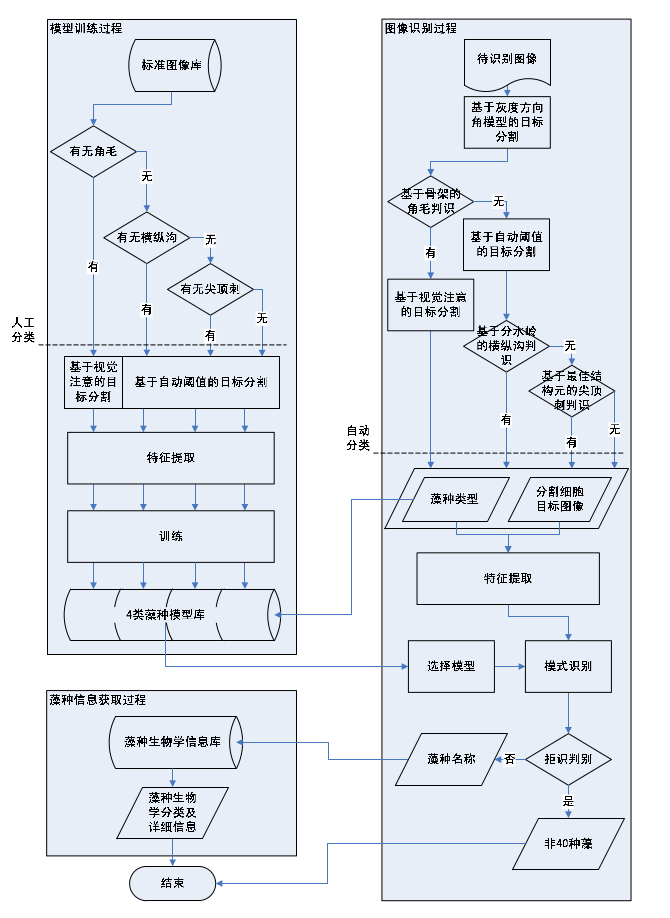
\includegraphics[width=0.5\textwidth]{流程图.png}
\end{frame}

%\section{实验室工作基础}

%\begin{frame}
%   \frametitle{各年级相关工作}
%   \begin{table}
%   \resizebox{0.8\hsize}{!}{$
%   \centering
%   \begin{tabular}{|c|c|c|}
%   \hline 
%   年级&姓名&课题 \\  
%   \hline
%   &史珊珊&基于分形理论的浮游植物显微图像识别研究\\ \cline{2-3} 
%   2009级&宋丽娜&基于多小波理论的浮游植物图像处理研究 \\ \cline{2-3}
%   &郑海永&基于生物形态学的有害赤潮藻显微图像诊断研究\\
%   \hline 
%   &吕梁 &有害赤潮数据采集与诊断系统的设计与实现\\ \cline{2-3} 
%   2010级&袁鹏&无角毛有害赤潮藻显微图像自动识别系统 \\ \cline{2-3}
%   &乔小燕&基于生物形态学的赤潮藻显微图像分割与特征提取研究\\
%   \hline
%   &鲍珊娟 &基于分形方法的有害赤潮显微图像识别研究\\ \cline{2-3} 
%   2011级&姜晓玲&基于变分水平集的赤潮藻显微图像分割方法研究 \\ \cline{2-3}
%   &郭春锋&中国海常见有害赤潮藻显微图像识别研究\\
%   \hline
%   2012级&张寒清&有害赤潮藻显微图像自动识别研究 \\
%   \hline
%   2013级&楚晶晶&基于显著区域检测和分水岭的无角毛类藻显微图像分割研究 \\
%   \hline
%   \end{tabular}$} 
%   \end{table}
%\end{frame}
 
\section{视觉显著性简介}

\subsection{是什么?}

\begin{frame}
  \frametitle{研究背景}
  \zhushadow{视觉显著性} 人类视觉系统用于指引注意力分配和视觉认知过程的生理机制
  \begin{figure}[!ht]
  \begin{minipage}[t]{0.2\textwidth}
  \centering
  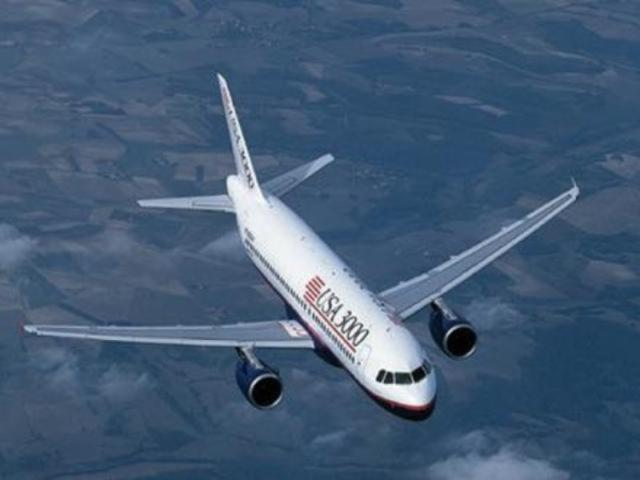
\includegraphics[width=1in]{11.jpg}
  \caption{原图}
  \end{minipage}
  \begin{minipage}[t]{0.2\textwidth}
  \centering
  
\includegraphics[width=1in]{11.png}
  \caption{真值图}
  \end{minipage}
  \begin{minipage}[t]{0.2\textwidth}
  \centering
  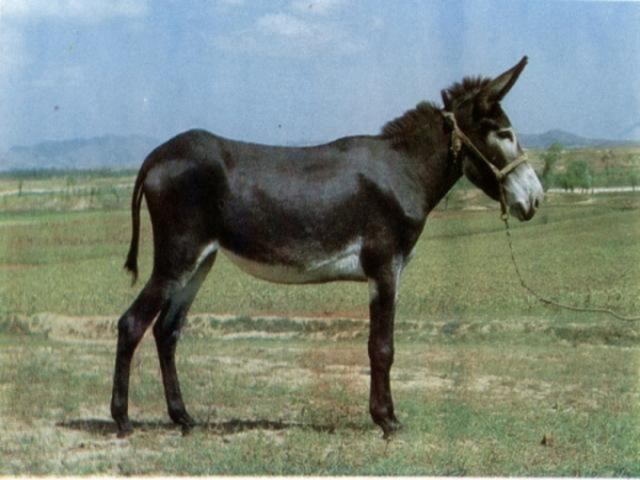
\includegraphics[width=1in]{14.jpg}
  \caption{原图}
  \end{minipage}
  \begin{minipage}[t]{0.2\textwidth}
  \centering
  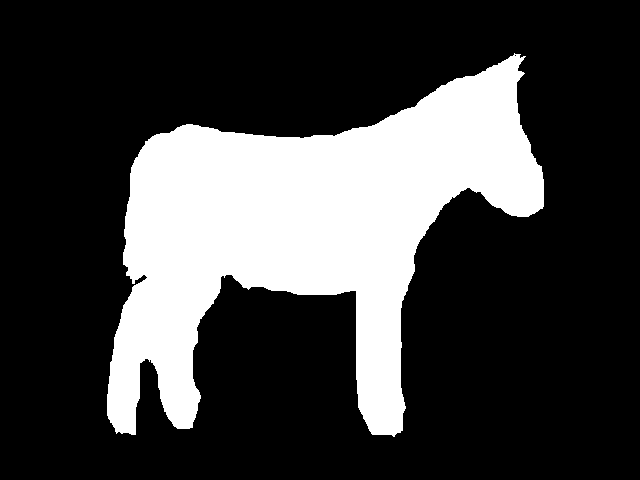
\includegraphics[width=1in]{14.png}
  \caption{真值图}
  \end{minipage}
  \end{figure}   
\end{frame}


%\begin{frame}
%  \frametitle{一般分类}
%  \begin{figure}[h]
%  \centering
%  \centerline{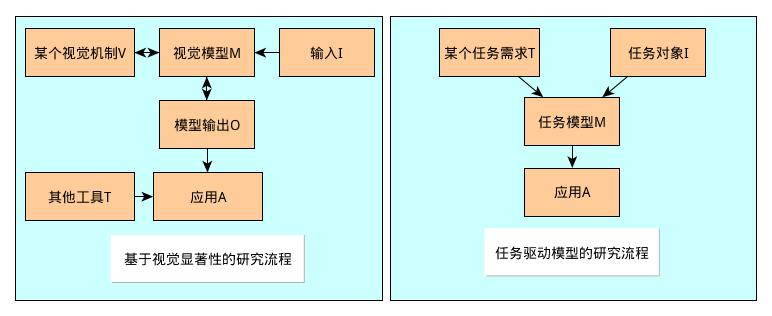
\includegraphics[width=4in]{流程图.jpg}}
%  \caption{基于视觉模型和任务驱动模型的研究流程比较}
%  \end{figure}
%\end{frame}


\subsection{为什么?}

\begin{frame}
  \begin{itemize}
  \item 显著性检测在计算机视觉领域是一个非常热的话题
  \item 研究视觉显著性是研究其他计算机视觉问题的基础
  \end{itemize}
\end{frame}

\subsection{怎么做?}

\subsubsection{代表性工作介绍}

\begin{frame}
  \frametitle{启蒙:Itti1998模型---最早提出的视觉注意模型}
  \begin{figure}[!ht]
  \begin{minipage}[t]{0.45\textwidth}
  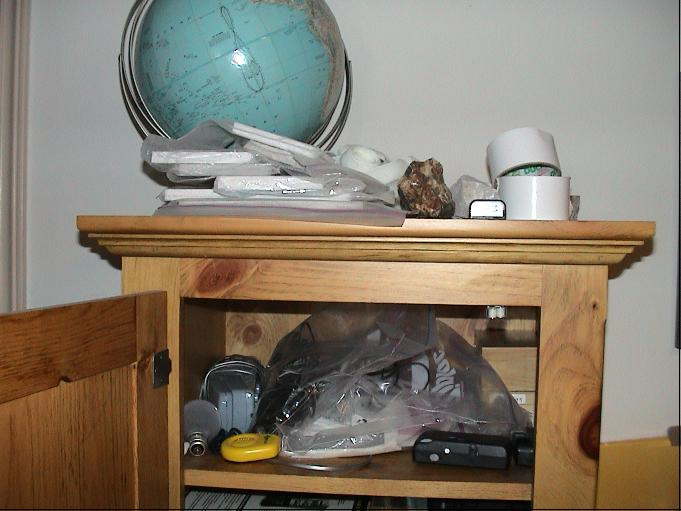
\includegraphics[width=2in]{IttiIMG.jpg}
  \caption{原图}
  \end{minipage}
  \begin{minipage}[t]{0.45\textwidth}
  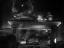
\includegraphics[width=2in]{IttiSM.png}
  \caption{显著图}
  \end{minipage}
  \end{figure} 
\end{frame}


\begin{frame}
  \frametitle{启蒙:Itti1998模型---最早提出的视觉注意模型}
  \centering
\includegraphics[width=2.5in]{model.png}
\end{frame}


\begin{frame}
  \frametitle{分支形成:Learning to Detect A Salient Object,CVPR 2007}
  \centering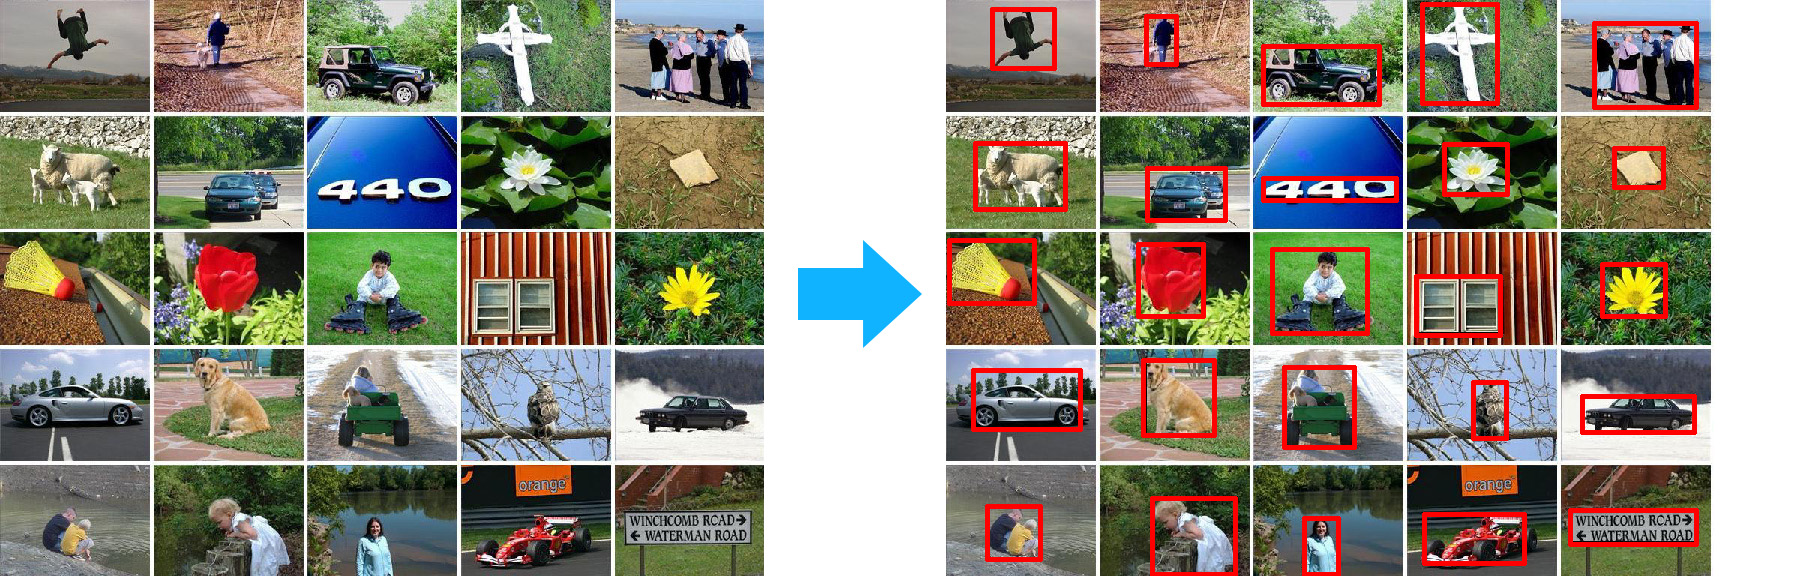
\includegraphics[width=4.5in]{MSRA.jpg}
\end{frame}


\begin{frame}
  \frametitle{分支形成:Frequency-tuned Salient Region Detection,CVPR 2009}
  \centering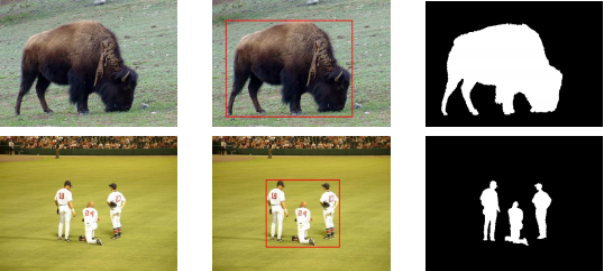
\includegraphics[width=3in]{FT.png}
\end{frame}

\subsubsection{我和师姐的工作}

\begin{frame}
  \frametitle{赵红苗的工作}
  \centering\includegraphics[width=3.5in]{zhm.eps}
\end{frame}


\begin{frame}
  \frametitle{我的工作}
  \begin{figure}[!ht]
  \begin{minipage}[t]{0.5\textwidth}
  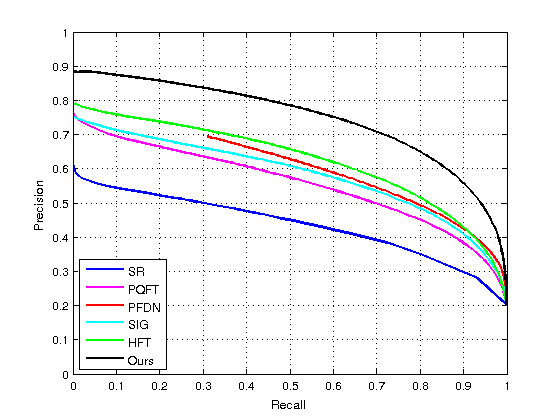
\includegraphics[width=2.5in]{PR_OTSU_1.2.png}
  \end{minipage}
  \begin{minipage}[t]{0.45\textwidth}
  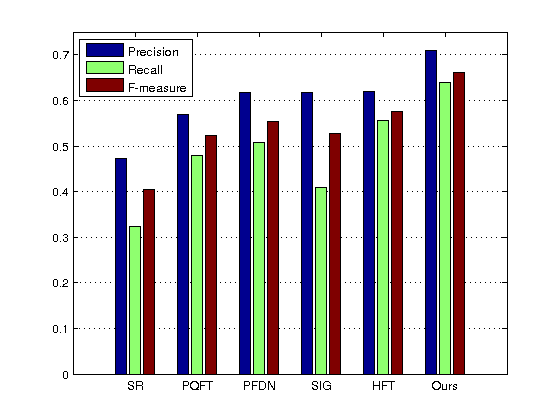
\includegraphics[width=2.5in]{PRF_OTSU_1.2.png}
  \end{minipage}
  \end{figure} 
\end{frame}


\begin{frame}
  \frametitle{科研计划}
  \begin{enumerate}
  \item 2014.10.01-2014.11.30:文献阅读,运行所有代码,寻找方向
  \item 2014.12.01-2014.12.31:进行实验
  \item 2014.01.01-2014.01.30:写论文并补充完善实验
  \item 2014.02.01-2014.02.15:修改论文
  \end{enumerate}
\end{frame}


\begin{frame}
  \vspace{2cm}
  \centering
  \zhushadow{\color{blue}\Huge{Thanks}}\\
  \vspace{1.5cm}
  \begin{flushright}
  \emph{\href{mailto:bingzh@ouc.edu.cn}{Yafei~Zhu}}\\
  \href{http://www.ouc.edu.cn}{Ocean University of China}\\
  \emph{2014.10}
  \end{flushright}  
\end{frame}
\end{document}


